\section{Simulating the bremsstrahlung cascade at all-order QCD}

In the second part of this project, the Monte Carlo integrator from the first part is supplemented with a parton shower, in order to add the effects of additional QCD bremsstrahlung produced by the final-state quark-antiquark pair. After a brief comment on parton showers and the kinematic limit in which it is possible to simulate this cascade at all orders in QCD, the use of the Monte Carlo integrator together with the Parton shower class provided is explained, discussing the change in final-state particles at the end. Finally, jets and jet clustering algorithms are introduced, together with histograms for the differential jet rates produced by the simulation, using as a baseline data produced with \textsc{Sherpa}.

\subsection{Parton Shower}

In the previous section, the leading-order squared matrix element, equation \eqref{eq:1-sqr-mat-element}, is quadratic on the QED coupling $\alpha$. The term “leading-order” implying, in this context, that we are dealing with the smallest possible power in the coupling, thereby neglecting further terms proportional to, e.g. $\alpha^{4}$. This coupling is not constant, however, and its value varies with the energy scale. Fortunately, the variation of the QED coupling at the energy scales relevant for the process here studied, is small: at low energy scales one has $\alpha \approx 1/137$, reaching $\alpha \approx 1 / 127$ at the scale of the Z boson.

Once the quark-antiquark pair is emitted, these accelerated color-charged particles can radiate gluons (\textit{bremsstrahlung}), which in turn can decay emitting more particles, giving rise to a “cascade”. 
\begin{wrapfigure}{r}{0.5\textwidth}
    \centering
    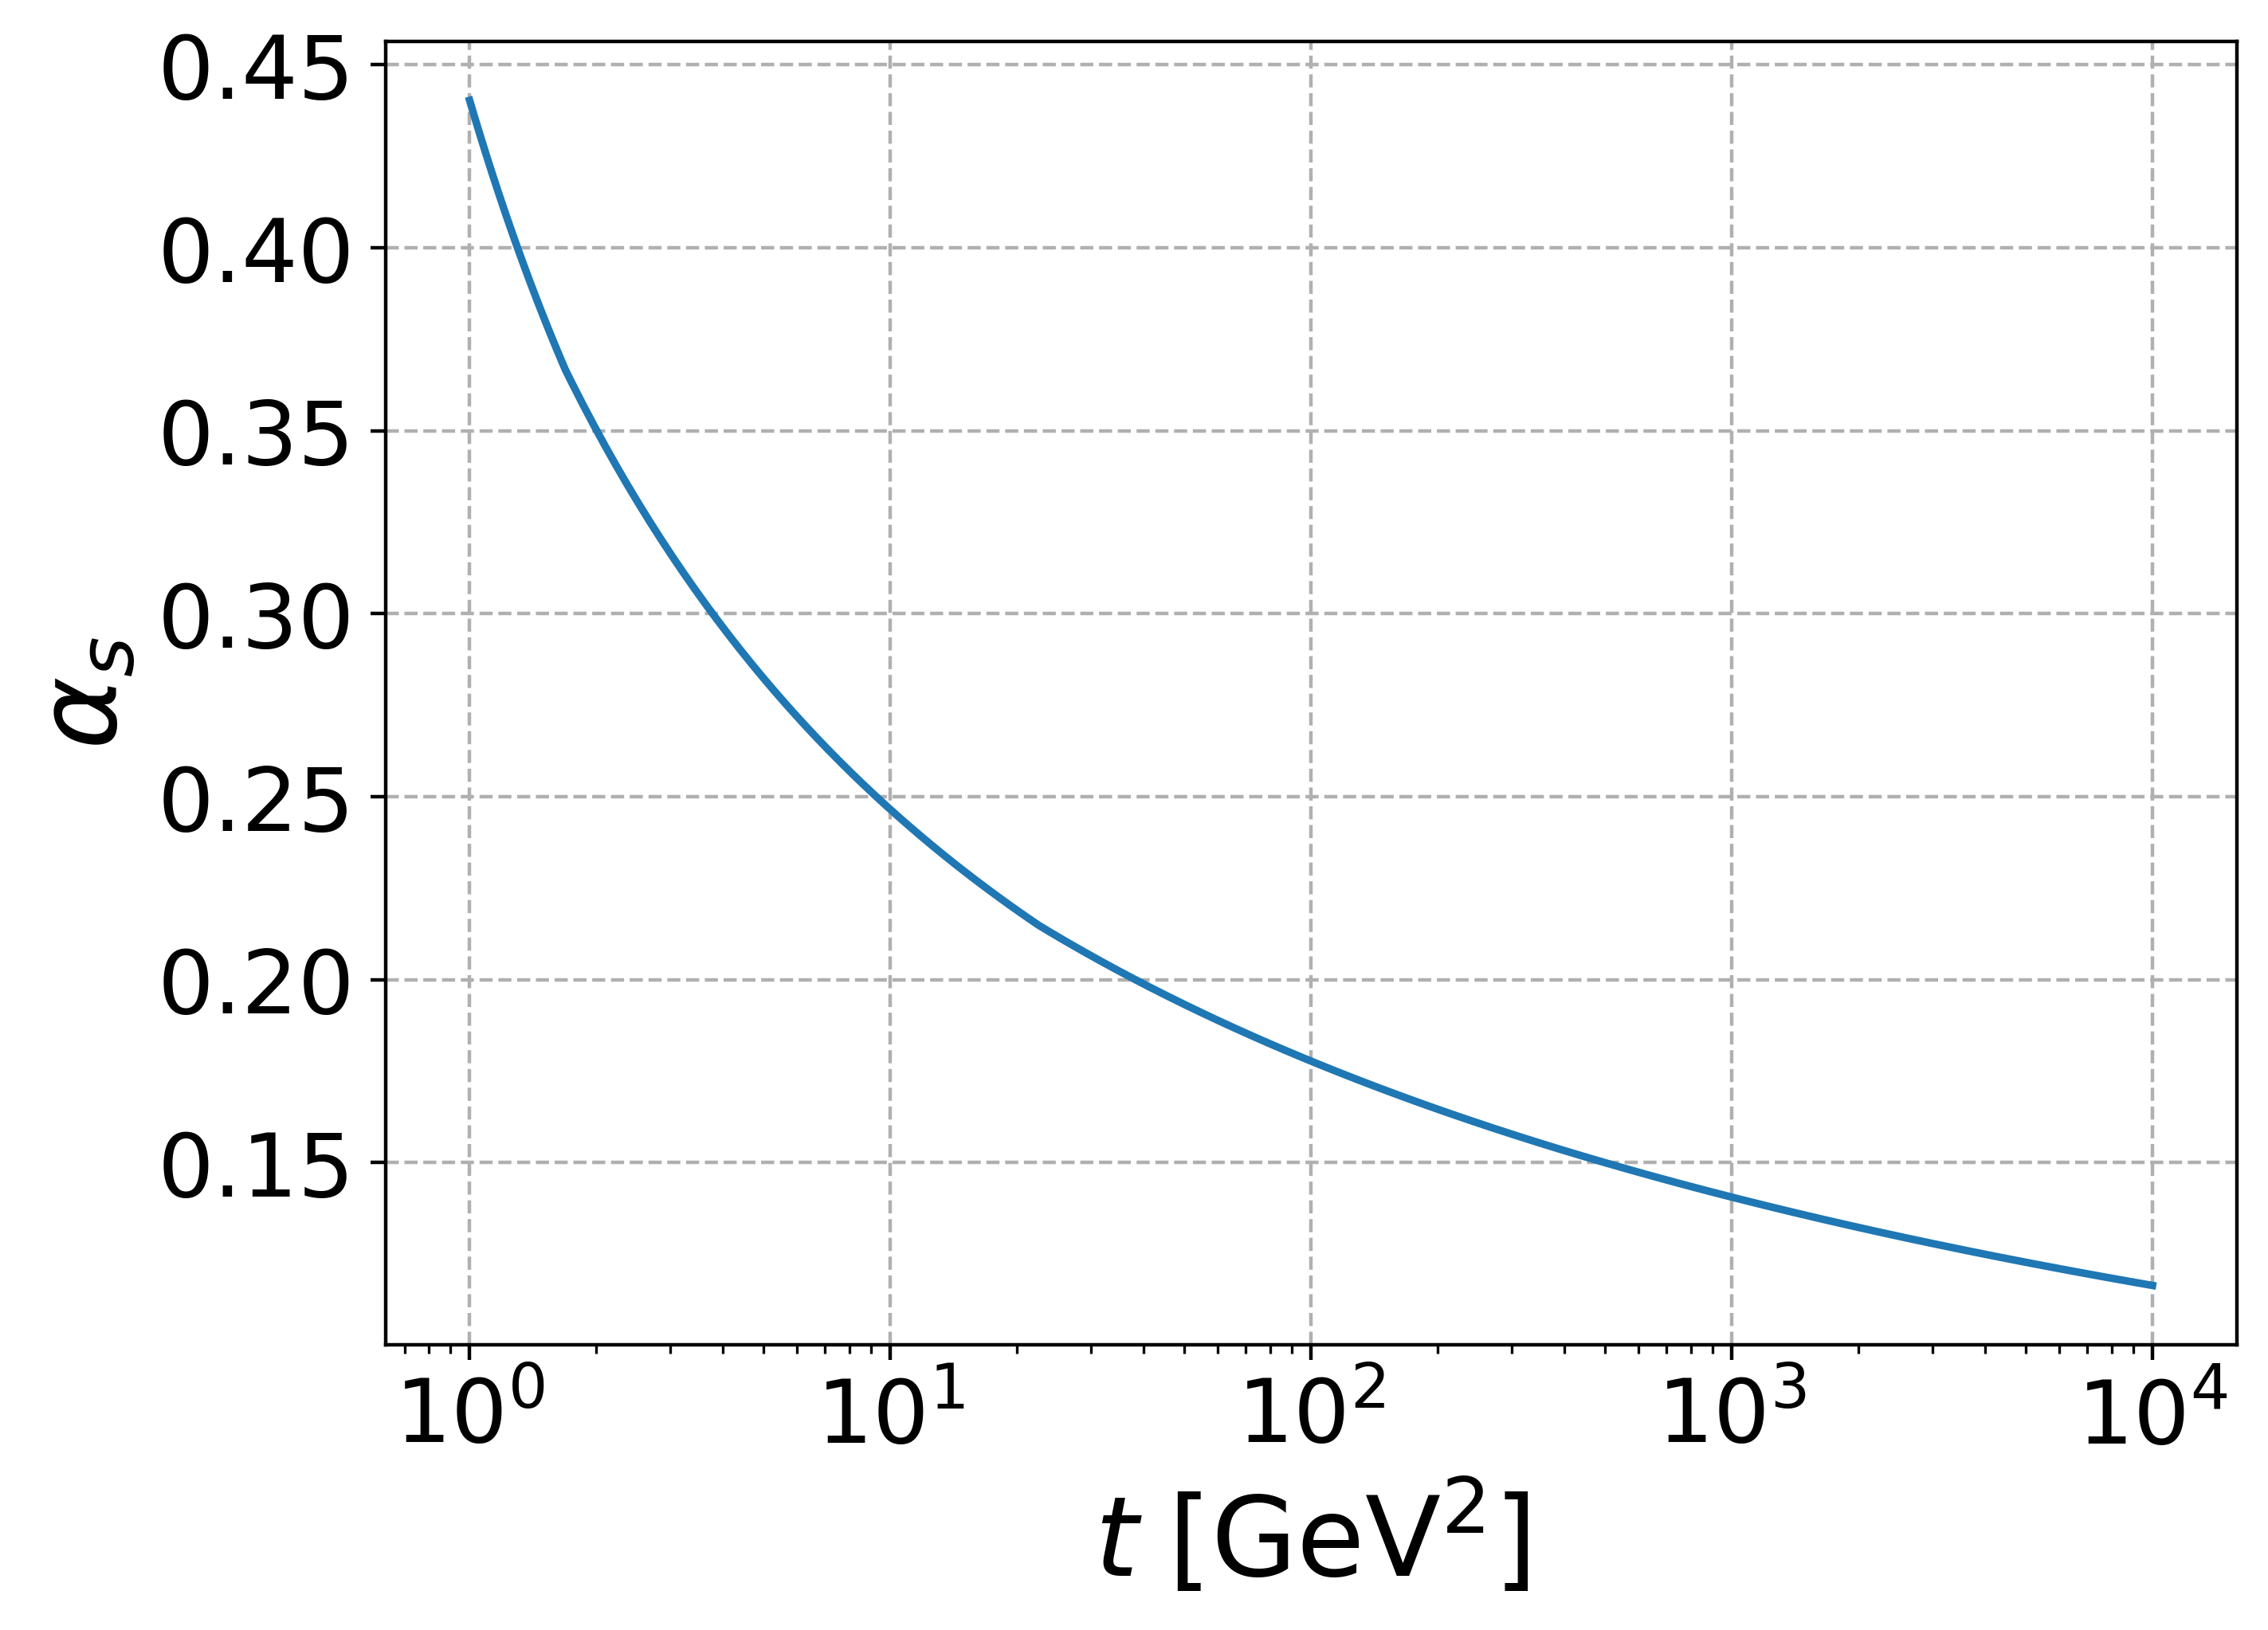
\includegraphics[width=0.5\textwidth]{figures/exercise2a.png}
  \caption{QCD coupling as a function of the squared energy scale.}
  \label{fig:2-alpha}
\end{wrapfigure}
This interaction between quarks and gluons is determined by the QCD coupling, $\alpha_{s}$, which, unlike the QED one, \textit{increases with decreasing energy scale}, see \autoref{fig:2-alpha}.\marginpar{Part a).} This means that some care is needed when trying to implement perturbation theory: \emph{if the energy scales become too small, the terms in the perturbative series cease to be smaller with increasing order}. 

One way to still apply perturbation theory and include this bremsstrahlung in the simulation, is to study this cascade in the kinematic limit where the emitted parton (i.e. a gluon or quark) is either collinear with its mother parton and/or soft, in other words, either the emission angle is small or the daughter's energy is small. In such case, the cross-section factorises into a part without the emission (the 2 -> 2 process of the previous section) and a universal emission factor, the latter enabling to treat subsequent emissions as a Markov Chain process, the simulation of which is called a “parton shower”. Furthermore, the restriction to small emission angles for the daughter particles gives rise to cone-shaped cascades, commonly referred to as \textit{partonic jets}.

\subsection{Monte Carlo integrator with parton shower}

Although the Monte Carlo integrator was developed from scratch, a \texttt{Shower} python class was provided for this project, the task being simply to “connect it” to the integrator.

An instance of \texttt{Shower} requires, for initialization, an instance of the class \texttt{AlphaS} and a lower cut-off scale $t_{0}$ (in $\text{GeV}^{2}$). The former is used to keep track of the “running” of the coupling $\alpha_{s}$ at different energy scales, while the latter represents a squared energy scale at which the emissions will be stopped when running the shower. Having created a single instance of it, the shower can be run with two arguments: (i) an \texttt{event}, consisting on a list of the incoming and outgoing particles, and (ii) the initial squared energy scale $t$. Then, the shower runs from the initial scale $t$ by generating emissions which lower the scale and modify in-place the \texttt{event} list (i.e. adds more particles to it), until the energy scale is below the cutoff, at which point the running stops.

The Monte Carlo integrator, being responsible for the cross-section factor without the emission, is precisely what is used to create the initial \texttt{event} list of particles. Each Monte Carlo point for the integrator has definite values of $s$, $\cos{\theta}$, $\phi$ and, performing a random sum over quark flavours, also a definite flavour q. From the kinematic variables, the momenta of the initial (electron-positron) and final particles (quark-antiquark) can be set, in the centre-of-mass frame, according to
\begin{equation}
    \begin{aligned}
        p_{\mathrm{e}^{-}} & = \frac{\sqrt{s}}{2} (1, 0, 0, -1), & \qquad p_{\mathrm{q}} & = \frac{\sqrt{s}}{2} (1, -\sin{\theta} \cos{\phi}, - \sin{\theta}\sin{\phi}, - \cos{\theta}) \\
        p_{\mathrm{e}^{+}} & = \frac{\sqrt{s}}{2} (1, 0, 0, +1), & \qquad p_{\bar{\mathrm{q}}} & = \frac{\sqrt{s}}{2} (1, +\sin{\theta} \cos{\phi}, + \sin{\theta}\sin{\phi}, + \cos{\theta}).
    \end{aligned}
\end{equation}
Besides the information of the momenta, the colour content of each particle also needs to be specified: the electron and the positron are colourless particles, the quark carries some colour and the antiquark carries the corresponding anti-colour. All this information is used to create instances of the \texttt{Particle} class (another class provided for the project), which form the elements of the initial \texttt{event} list.

Hence, the algorithm for the parton shower consists of sampling $N$ Monte Carlo points with the integrator, using the information of the kinematic variables and quark flavour to create one \texttt{event} per Monte Carlo point, to then pass these events to the shower, which modifies each of them in-place to yield events with final-state particles in them.

Following the above algorithm, the Monte Carlo integrator for a fixed beam distribution at the mass of the Z boson ($f(s) = \delta(s - M_{\mathrm{Z}}^{2})$) was used to generate 1,000 Monte Carlo points, which corresponded to the same number of events for which the parton shower was run. The cutoff scale was set to $t_{0} = 1 \text{GeV}^{2}$ and the initial scale at $t = M_{\mathrm{Z}}^{2}$. For each of these events, the number of final-state particles was counted and weighted according to its Monte Carlo weight, giving a \marginpar{Part c).}\emph{weighted average of 5.25(6) particles}.

\subsection{Jets and the Durham algorithm}

In the initialization of the parton shower discussed in the previous section, one of the required parameters is the energy scale cutoff $t_{0}$, below which the perturbative method no longer applies and the running of the shower is stopped. This unphysical parameter is introduced because the probabilities to emit additional quark or gluons at small angles or small energies diverges. However, in doing so, quantities like the number of particles after showering are ill-defined, as they depend on the choice of cutoff. At the same time, actual experiments have a limited resolution, which gives the possibility that additional collinear or soft partons are emitted, with the experimental signature being left unchanged.

In order to address both of these issues, jet algorithms have been developed. These algorithms cluster particles into jets that are well-separated, allowing for well-defined comparisons between experimental data and theory calculations.

For clustering the particles, two generic types of algorithms are commonly used: (i) cone algorithms and (ii) sequential recombination algorithms. In this project, the jet algorithm implemented for the analysis of the final state is the \textit{Durham $k_{T}$ algorithm}, which is of the second kind. This (final state) jet finding algorithm consists of the following:
\begin{enumerate}
    \item For each pair $(i, j)$ of final-state particles, compute the distance measure
    \begin{equation}
        y_{i j} = \frac{2 \text{min}(E_{i}^{2}, E_{j}^{2}) (1 - \cos{\theta_{ij}})}{Q^{2}},
    \end{equation}
    where $E_{i}$ is the energy of the $i$-th particle, $\theta_{i j} = \langle \mathbf{p}_{i}, \mathbf{p}_{j} \rangle$ is the angle between the spatial momenta, and $Q^{2}$ is a reference scale which, for this project, corresponds to the squared mass of the Z boson.

    \item Determine the pair of particles $(i, j)$ with the minimum $y_{i j}$ and combine them, i.e., sum their (four-)momenta.

    \item Repeat until all final-state particles are clustered into jets.
\end{enumerate}
The result of the above algorithm is a series of splitting scales, corresponding to the minimum values $y_{i j}$ found at each iteration. These splitting scales can then be used to quantify the contributions to the cross-section from different numbers of jets.

After implementing the Durham $k_{T}$ algorithm to cluster the final-state particles, an analysis of 1 million of events was carried out: The events were created using the Monte Carlo integrator at fixed beam energy, $s = M_{Z}^{2}$, for obtaining the initial and final-state particles properties, such as momentum and quark flavour, together with the Monte Carlo weights for each differential cross-section. The parton shower was then run for each of these events with a cutoff scale of $t_{0} = 1 \,\text{GeV}^{2}$ and an initial scale $t = M_{Z}^{2}$. The results can be seen in \autoref{fig:jet1} and \autoref{fig:jets}, where the results of the simulator are compared to those of \textsc{Sherpa} for differentials from 2 $\to$ 3 up to $5 \to 6$.

\begin{figure}[ht!]
    \centering
    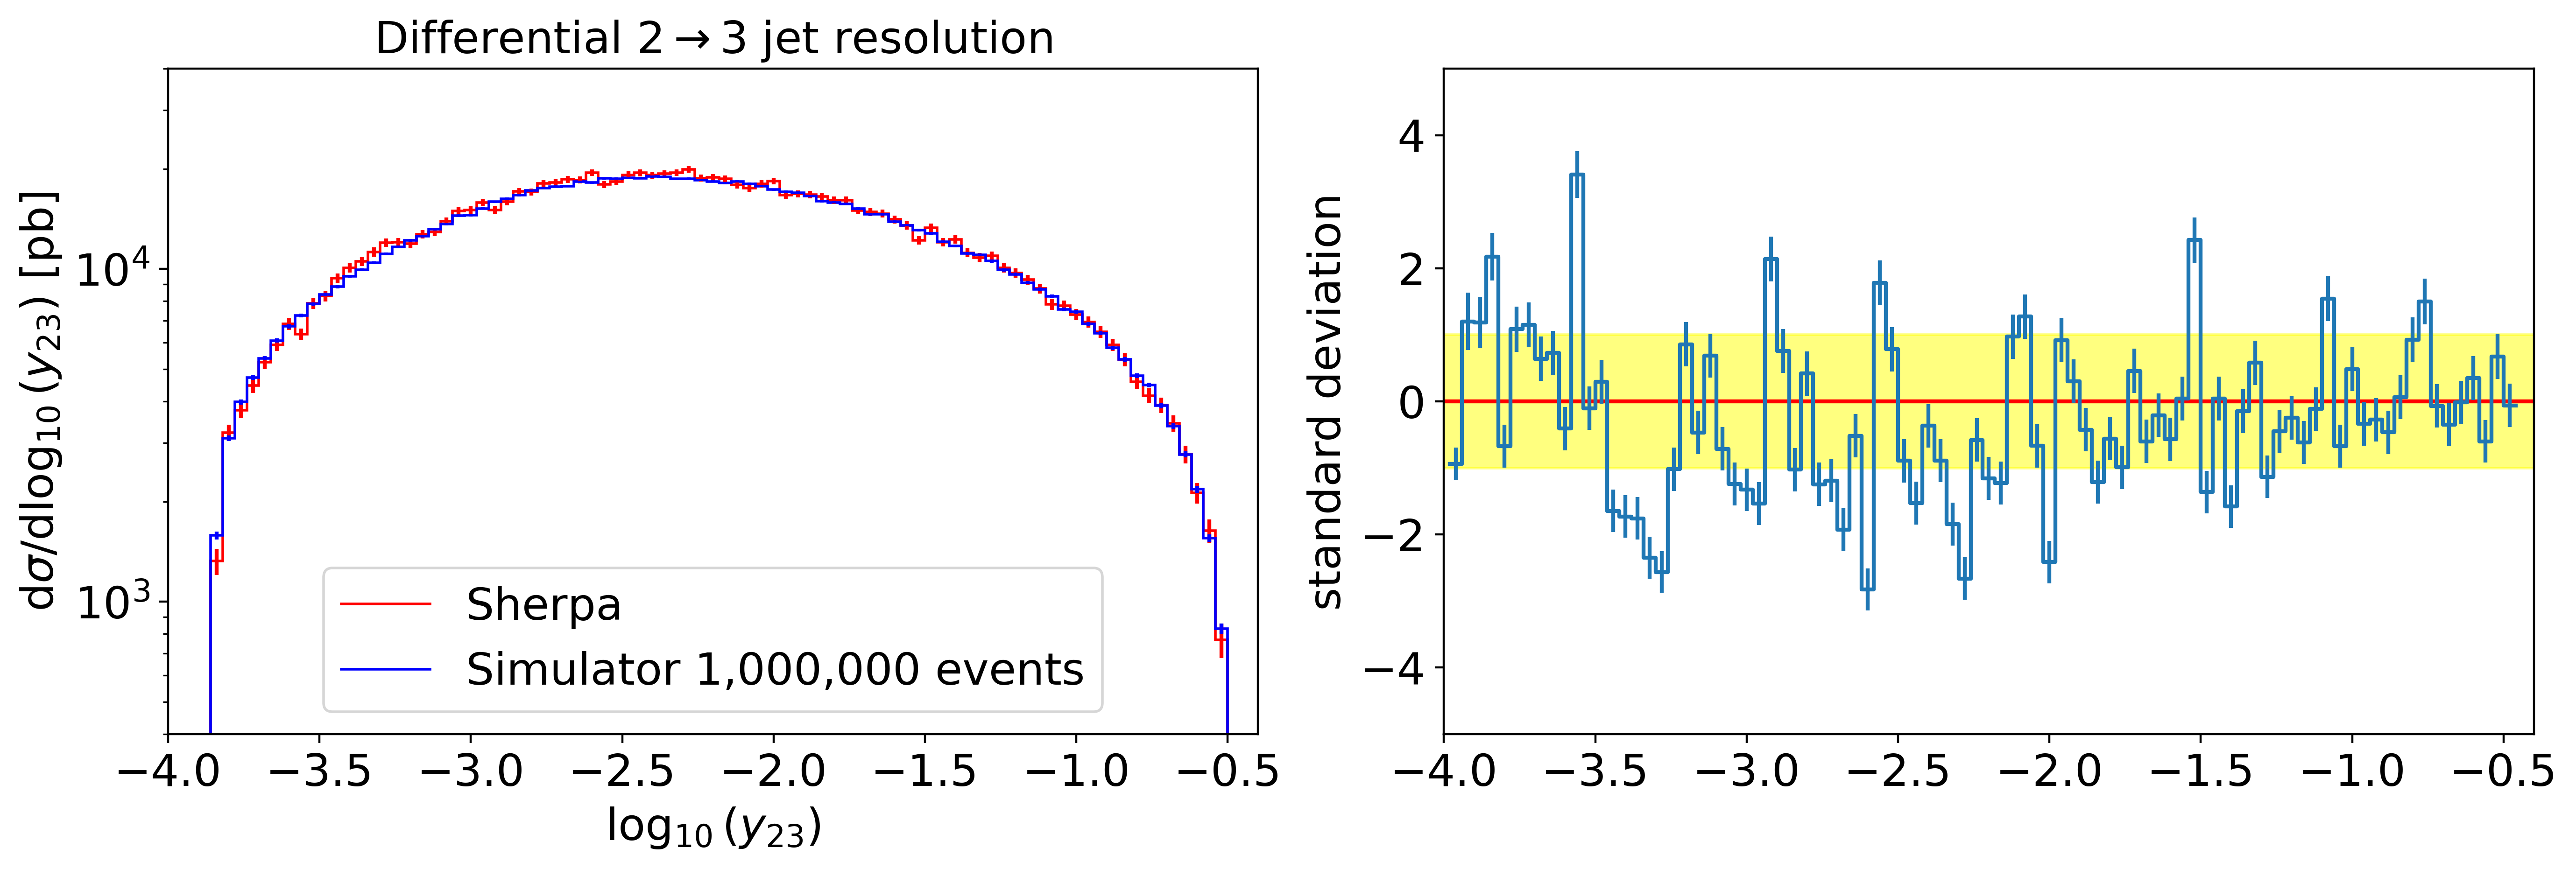
\includegraphics[width=\textwidth]{figures/jet_histo_1.png}
    \caption{}
    \label{fig:jet1}
\end{figure}

\clearpage

\begin{figure}[ht!]
    \centering
    \begin{subfigure}[t]{\textwidth}
        \centering
        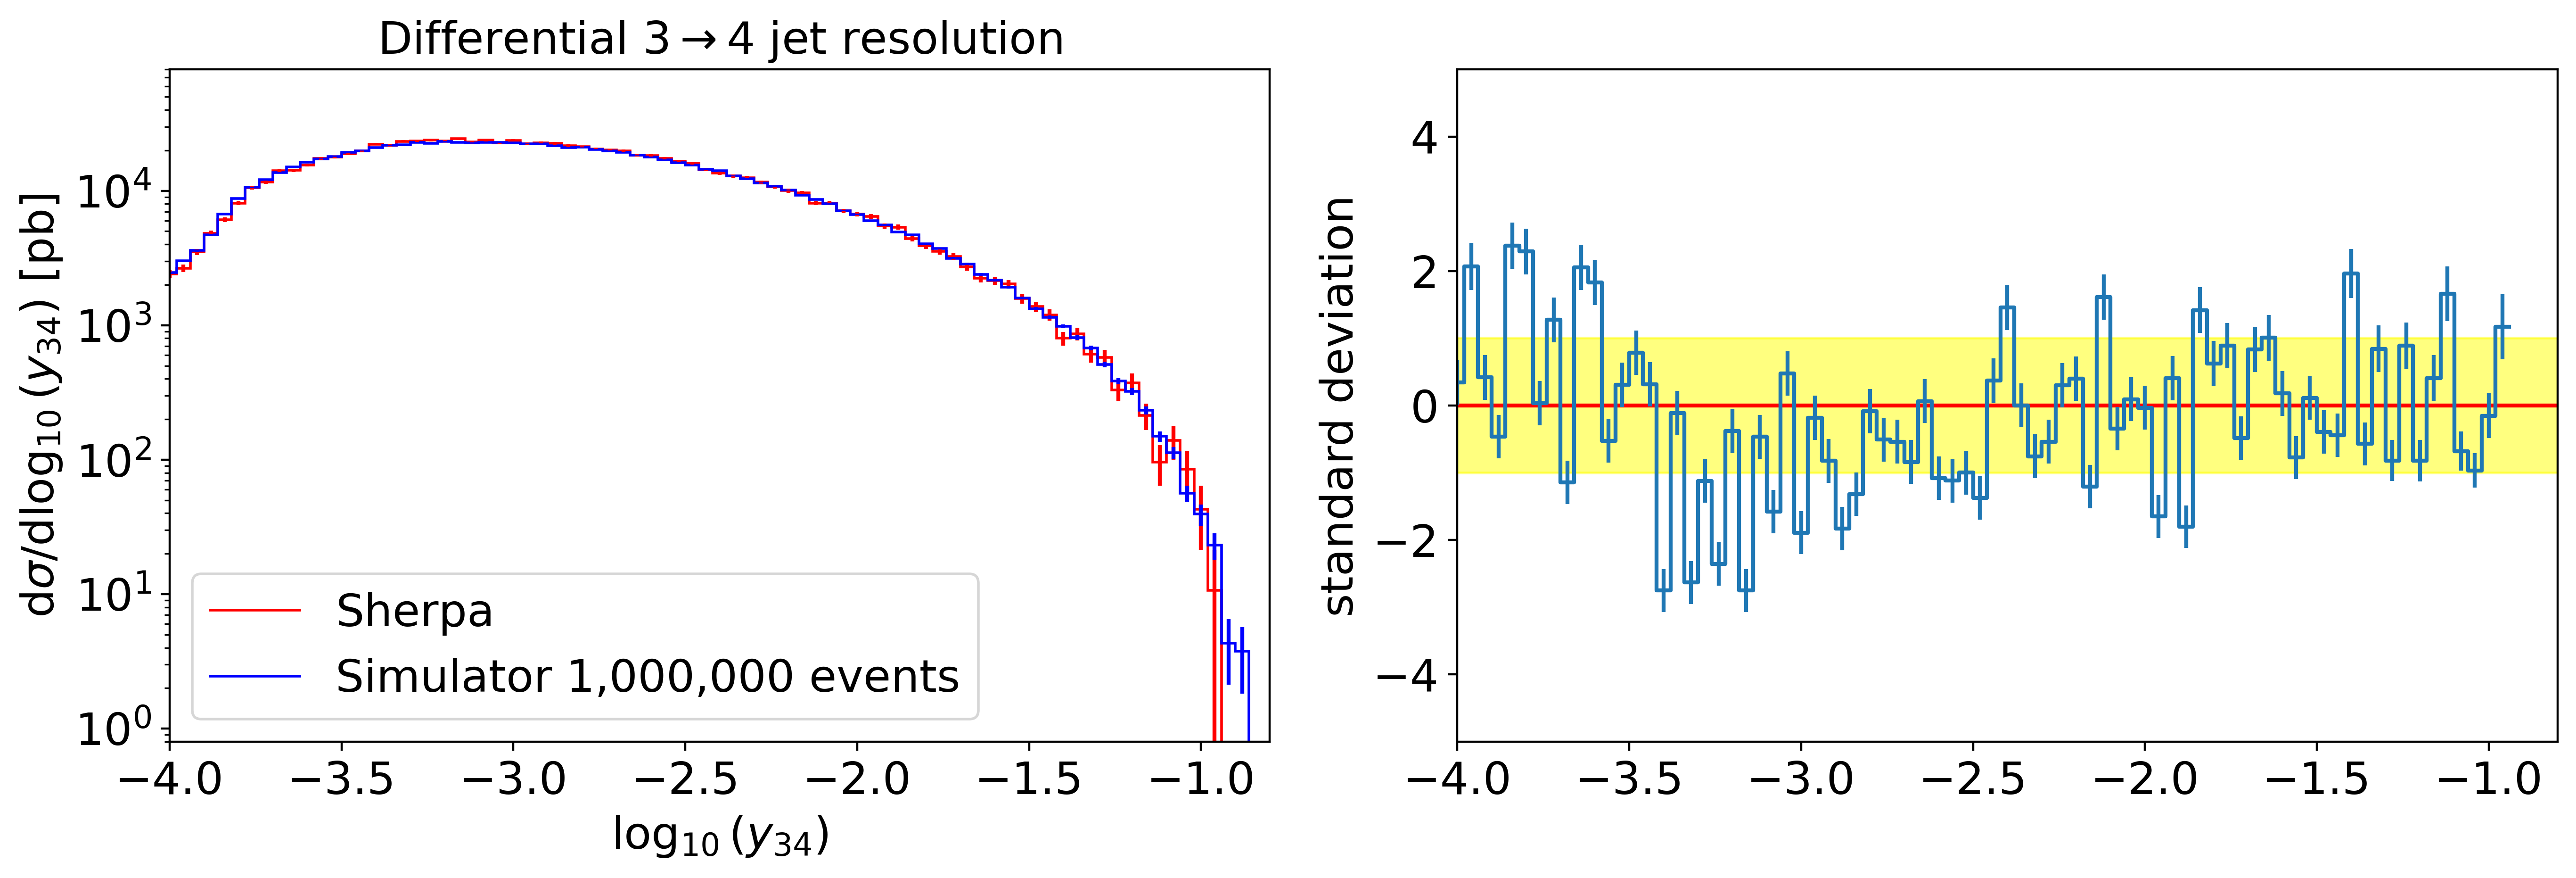
\includegraphics[width=\textwidth]{figures/jet_histo_2.png}
        \caption{}
        \label{fig:jet2}
    \end{subfigure}
    \hfill
    \begin{subfigure}[t]{\textwidth}
        \centering
        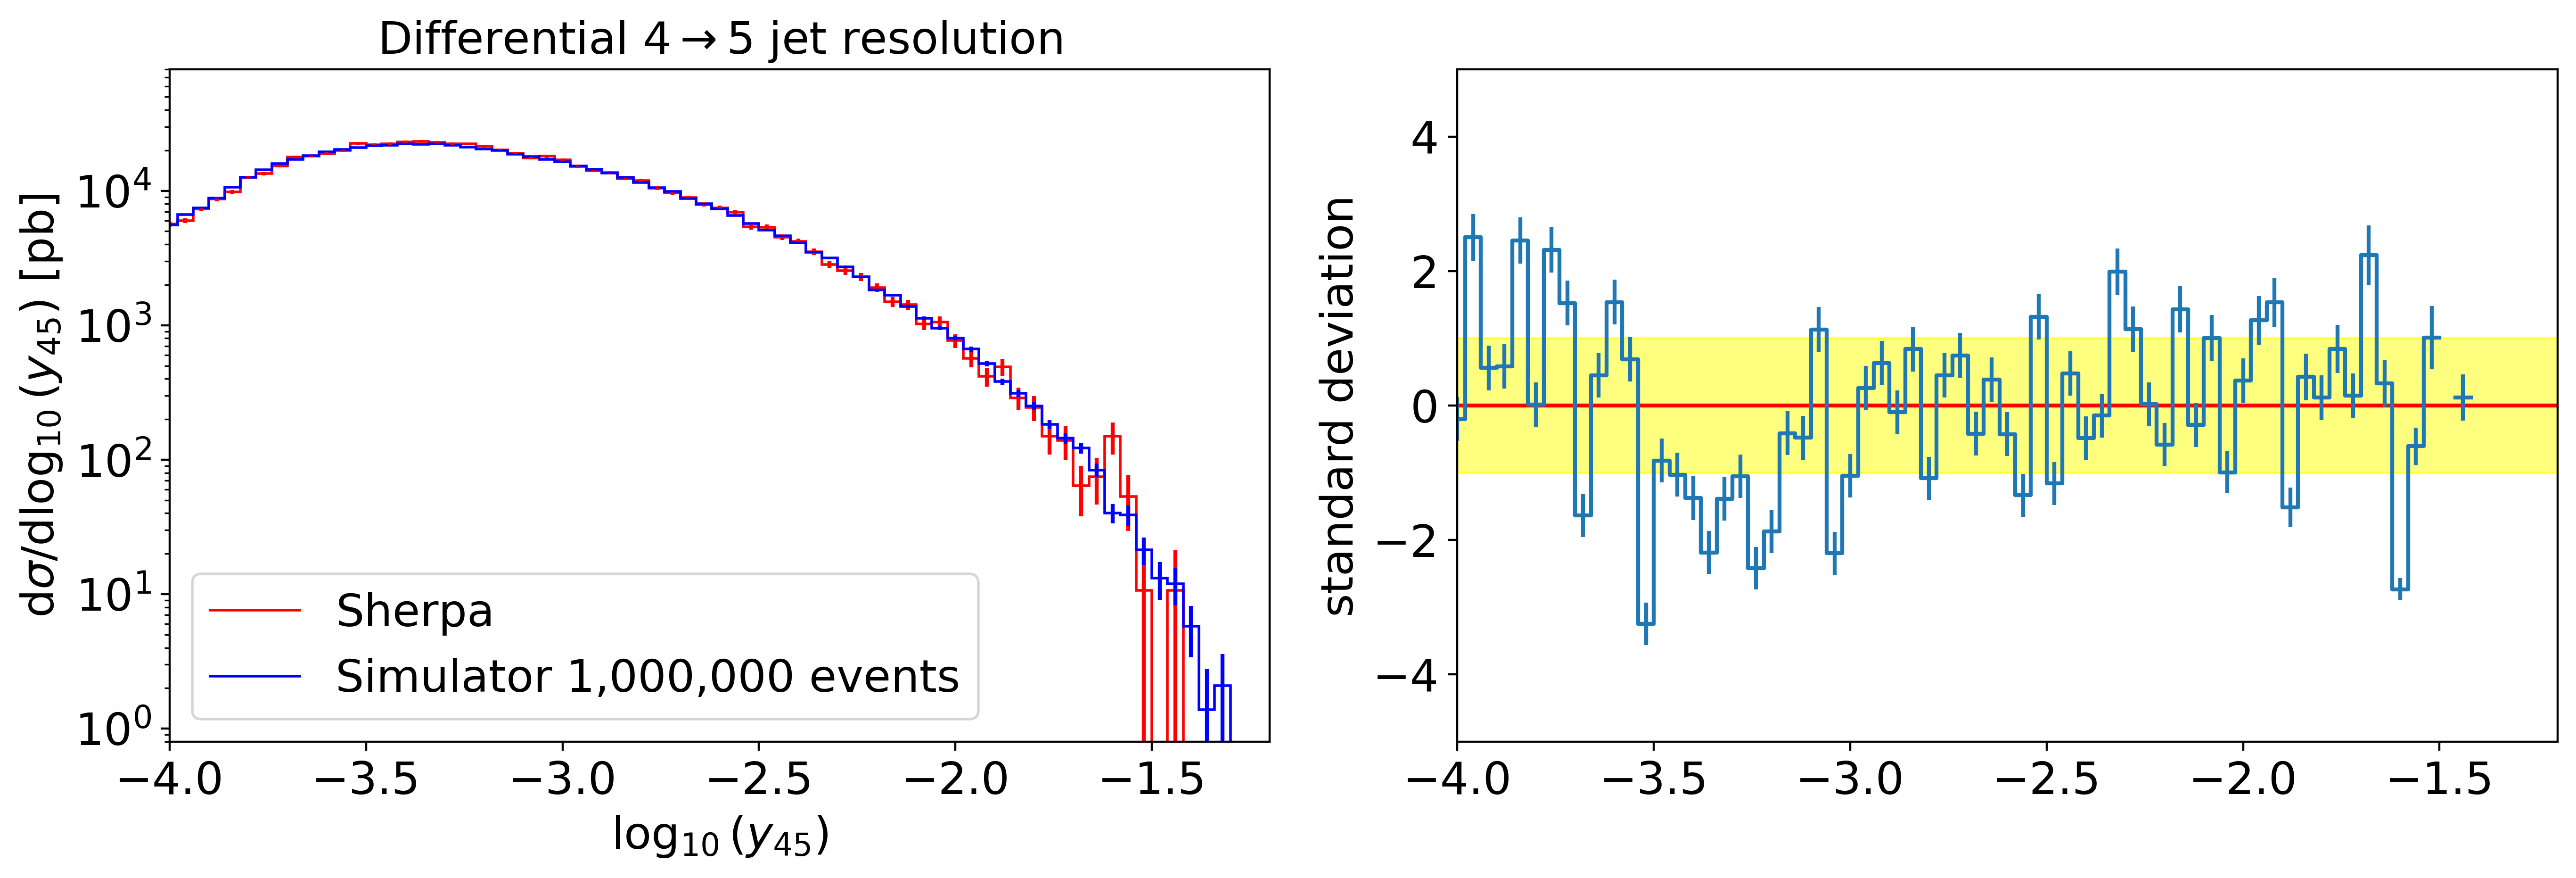
\includegraphics[width=\textwidth]{figures/jet_histo_3.png}
        \caption{}
        \label{fig:jet3}
    \end{subfigure}
    \hfill
    \begin{subfigure}[t]{\textwidth}
        \centering
        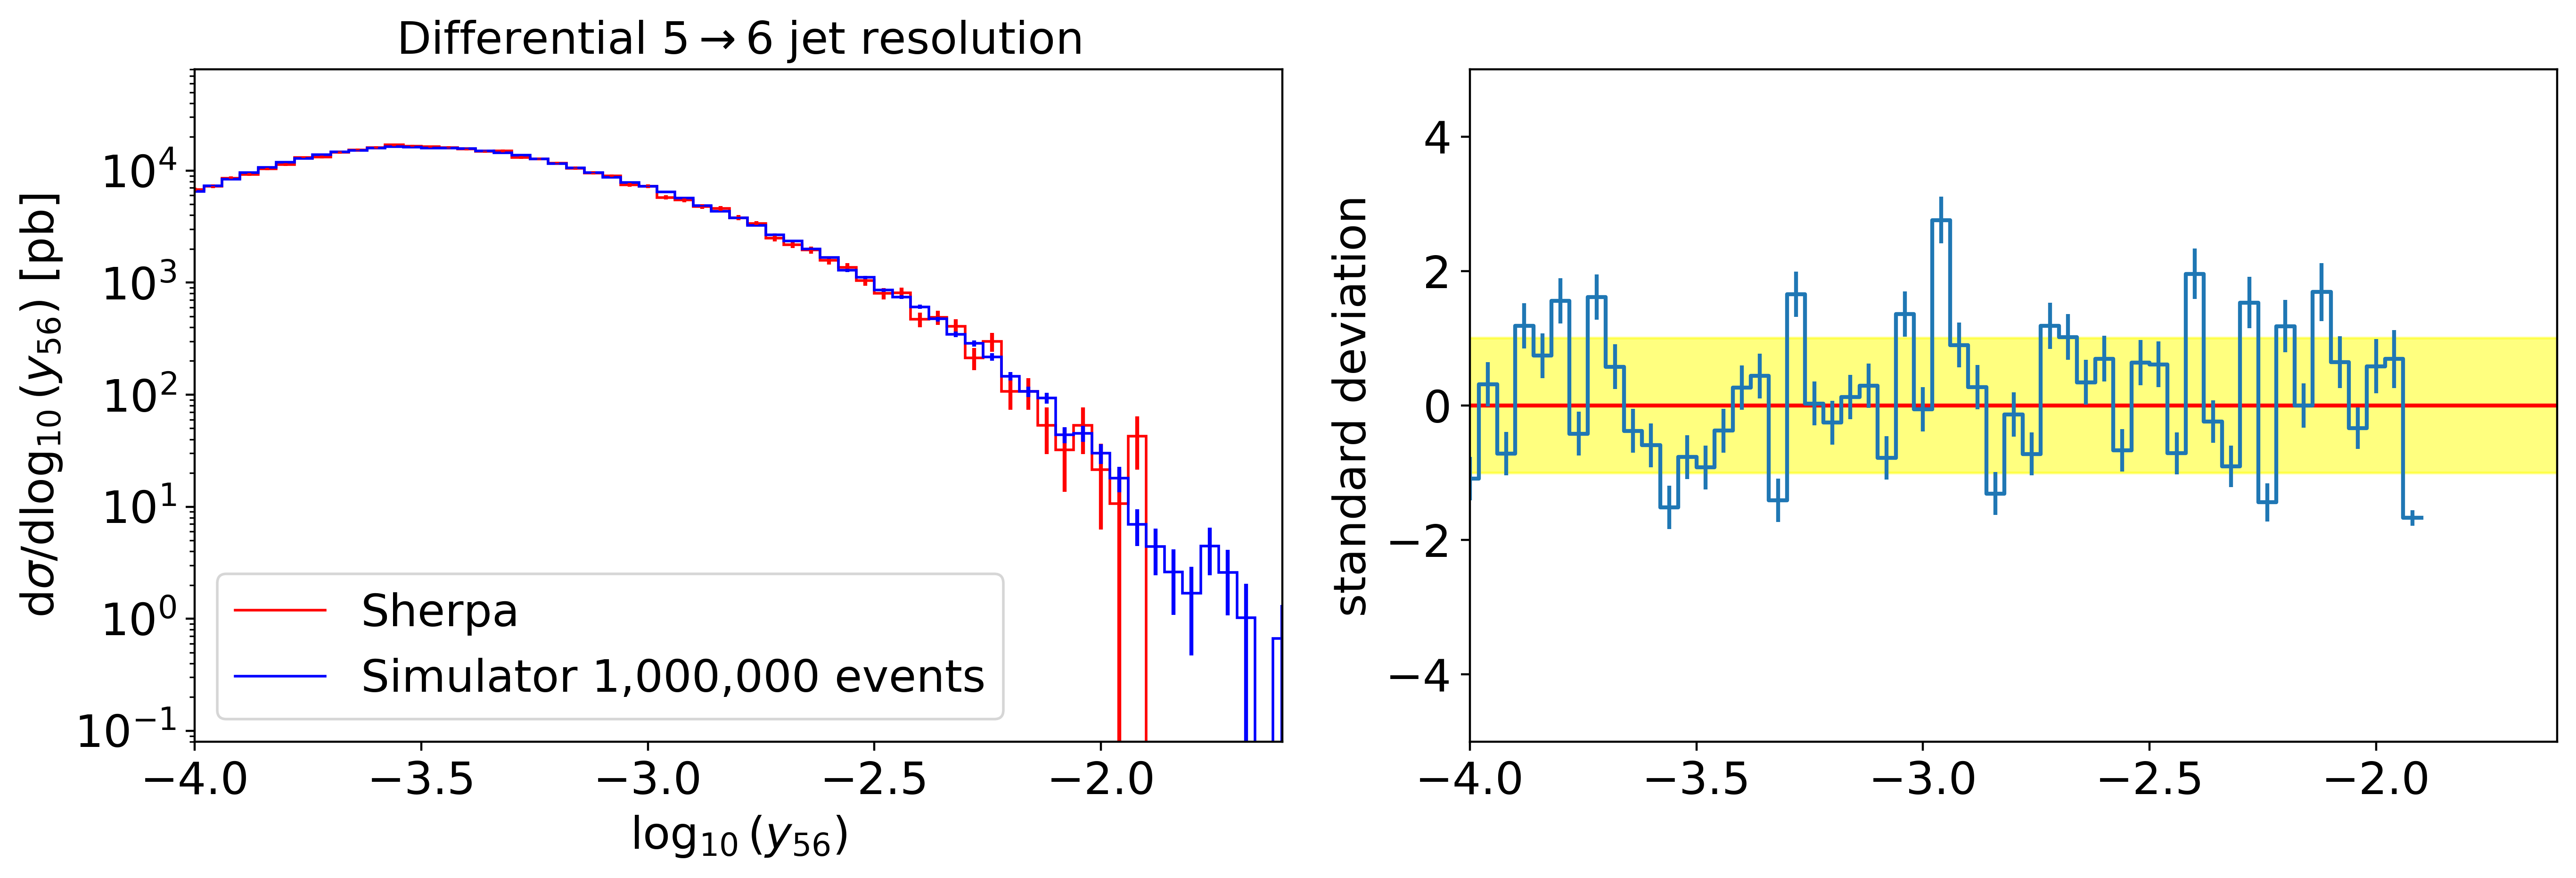
\includegraphics[width=\textwidth]{figures/jet_histo_4.png}
        \caption{}
        \label{fig:jet4}
    \end{subfigure}
    \caption{Jet resolution for several differentials. The plots on the right are the associated errors, in standard deviations, to the values of \textsc{Sherpa}.}
    \label{fig:jets}
\end{figure}